\chapter{Implementierung}
Die grundlegenden Funktionen dieser Arbeit sollen das Erstellen von Veranstaltungen und Benutzern, die Zuweisung untereinander und die Kompatibilität mit mobilen Endgeräten umfassen. Wie diese Funktionen mit Hilfe von modernen Webtechniken implementiert wurden, wird hier beschrieben.

\section{Problembeschreibung}
Zur Idee dieser Bachelorarbeit liegt folgende Frage zugrunde:

\begin{quote}
	Kann man eine App entwickeln, in der man zu einer bestimmten Veranstaltung beliebig viele Teilnehmer hinzufügen, deren spezifischen Anmeldedaten hinterlegen und später schließlich verteilt mit beliebig vielen Helfern (mobil) daran arbeiten kann? 
\end{quote}

Diese Fragestellung ist deshalb interessant, weil diese App in erster Linie im Oktober am freideutschen Jugendtag verwendet werden soll. Dort werden über 4000 Pfadfinder erwartet, die aus Deutschland, Schweiz und Österreich stammen und zu verschiedenen Zeiten an- und abreisen. Außerdem benötigen einige Gruppen besondere Materialien (vorwiegend verschieden lange Holzstangen für den Bau diverser Zelte), die vorher von den Helfern organisiert werden müssen.\par

\subsection{Identifizierung des Problems}
Bei dem Gedanken eine App zu entwickeln steht man oft vor der Entscheidung für welche Plattform man denn entwickeln möchte: Linux, Windows, OS X, iOS, Android, Windows Phone, Blackberry OS, \dots \ Doch das würde voraussetzen, dass alle Benutzer dieser App das gleiche Betriebssystem benutzen, was eine schlechte Annahme ist, da dies nicht der Realität entspricht.\par

Wieso also nicht für alle Plattformen gleichermaßen entwickeln? Dank dem Google Projekt \glqq HTML5 Rocks\grqq{}\cite{html5rocksmain} und vielen weiteren Personen ist \emph{HTML5} in aller Munde und somit gibt es tatsächlich die Möglichkeit jedes Betriebssystem mit einer einzigen Web-App abzudecken.

\paragraph{Definition Webanwendung} 
Eine Webanwendung (auch \emph{Web-App} genannt) ist eine Anwendung, die vollständig in einem Browser ausführbar ist. Da sie (fast) vollständig auf einem Webserver ausgeführt wird, ist das zugrunde liegende Übertragungsprotokoll \emph{HTTP}.\par

Web-Apps bieten den Vorteil, dass sie in jedem modernen Browser ausgeführt werden können, ohne, dass spezielle Programmiersprachen erlernt und angewendet werden müssen. Interessant sind diese Anwendungen, da sie auch auf Smartphones und Tablets ausgeführt werden können ohne sie vollständig auf die jeweilige Plattform portieren zu müssen.

Damit sind die zugrunde liegenden Programmiersprachen festgelegt. Mit der Wahl des Open Source Frameworks \emph{cakePHP} \cite{cakePHP} stehen auch serverseitig \emph{PHP5} und clientseitig \emph{JavaScript} als weitere Sprachen fest. Als Datenbank wird \emph{MySQL} gewählt und für den Webserver kommt \emph{Apache} zum Einsatz, beides ist durch das Entwicklerpaket \emph{XMPP} gegeben.

\subsection{Beschreibung der Umgebung}
Da eine Web-App eine Internetverbindung (mindestens zum initialen Laden) benötigt, muss gesichert sein, dass diese auch zur Verfügung steht. Meine Webanwendung soll zuerst am Meißnerlager 2013 am Hohen Meißner verwendet werden, wo im Allgemeinen eine schlechte Internetanbindung zwischen den Bergen zu erwarten ist, allerdings hat ein großes Telekommunikationsunternehmen die Versorgung durch einen eigenen Funkmast zugesichert. Somit ist garantiert, dass die App dort verwendet werden kann.

\section{Struktur der Webanwendung}
Für die Grundstruktur wurde das Open Source Framework cakePHP verwendet. Diese verwendet für eine klare Trennung der Logik und dem Design das Entwurfsmuster \emph{Model View Controller}.

\subsection{Entwurfsmuster: Model View Controller}

Befasst man sich mit dem Entwickeln von modernen Webseiten, Apps oder ähnlichen Projekten, so stößt man direkt auf das Muster zur Strukturierung als Model View Controller (deutsch: Modell-Präsentation-Steuerung, kurz: \emph{MVC}). Dieses Muster kapselt die drei Elemente voneinander und ermöglicht dadurch, dass Änderungen einfach implementiert werden können.

\begin{figure}[!ht]
	\centering
	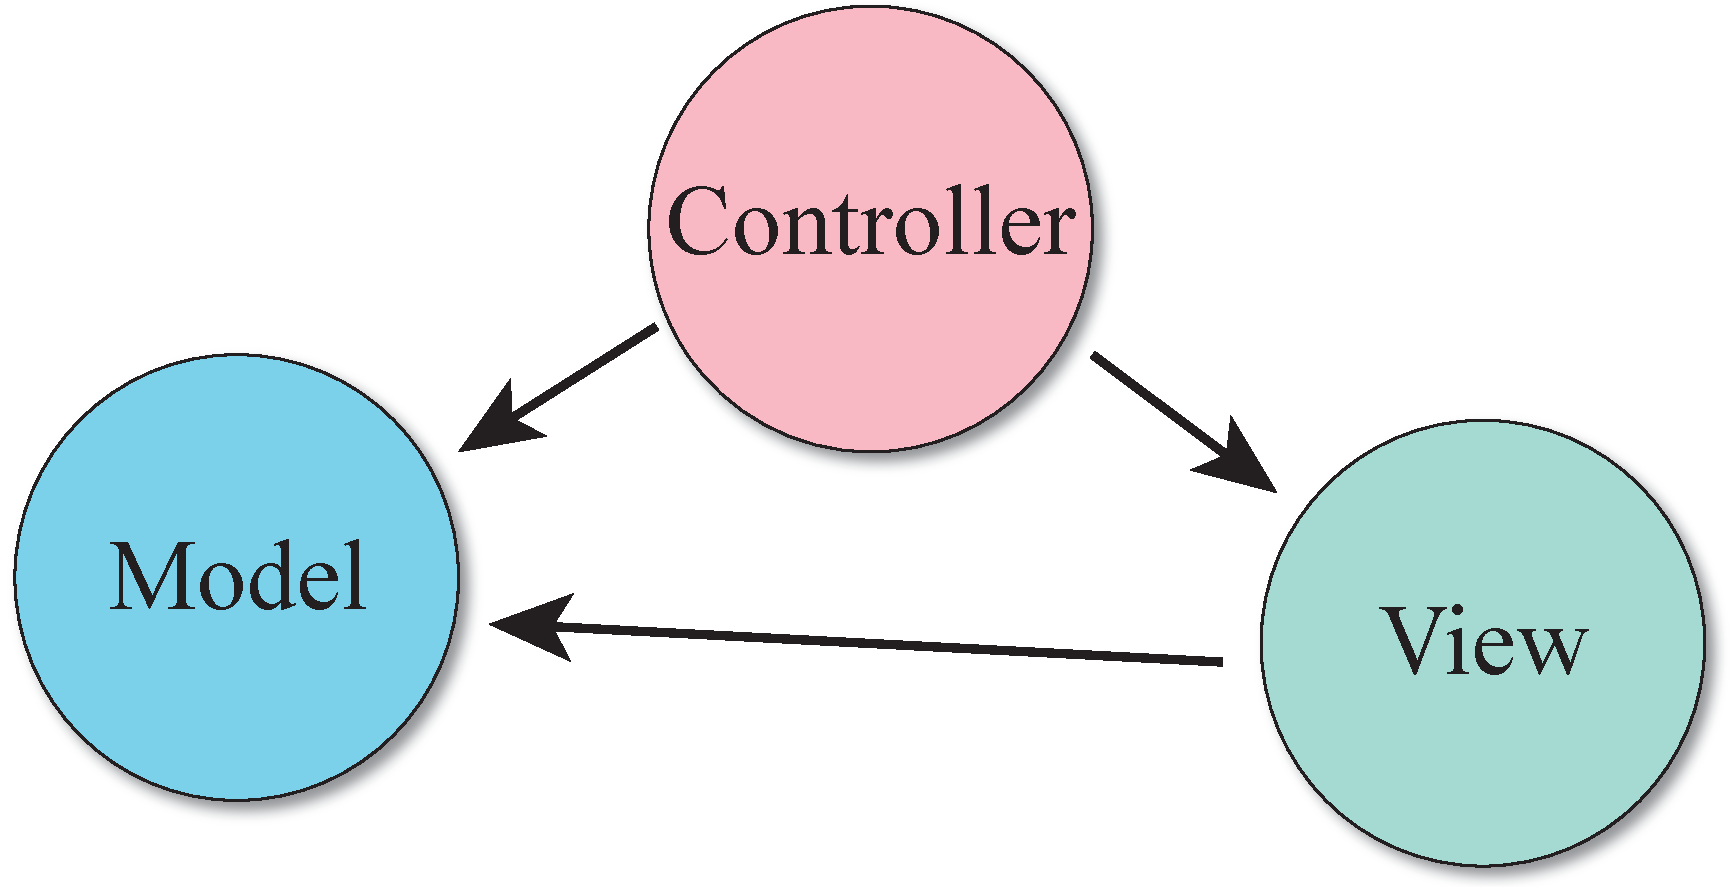
\includegraphics[width=10cm]{fig/mvc}
	\caption{Direkte Assoziationen zwischen Model, View und Controller}
\end{figure}

\underline{Model:}\\
Verantwortlich für alles, was die Daten eines bestimmten Models angeht. In dieser Anwendung ist dieser Bereich für Interaktionen, Gültigkeit und Auswertung verantwortlich und repräsentiert hier zum Beispiel eine Veranstaltung, ein Benutzer, Statistiken oder Koordinaten der Benutzer.

\underline{View:}\\
Generiert das Aussehen einer bestimmten Seite. Hier wird vorwiegend mit gängigen Webformaten, wie HTML, PHP und JavaScript gearbeitet. Ein View kann auf die Daten zugreifen, die ihm der Controller liefert und diese dann anschaulich darstellen. Dadurch muss sich ein View nicht darum kümmern woher er seine Informationen zusammensuchen muss, sondern bekommt garantiert, dass diese vom Controller bereit gestellt wurden. Hierbei können verschiedene Views für verschiedene Geräte erstellt werden und erlauben so einfach eine mobile Seite zu generieren.

\underline{Controller:}\\
Hier findet die gesamte Logik und Aufbereitung der Daten statt, die später dem Benutzer im View angezeigt werden sollen. Sämtliche Datenbankabfragen, Berechnungen oder Ähnliches werden hier durchgeführt und dem Model / View bereitgestellt. Für jedes Objekt existiert ein eigener Controller, diese werden \emph{EventsController}, \emph{UsersController} etc. genannt. \\
In diesem Framework ist jede Funktion direkt mit den Views verknüpft, das heißt definiert man im EventsController eine Funktion namens \emph{index()}, so stellt dies eine Seite der Webanwendung dar, die mit \emph{http://localhost/Events/index} aufgerufen werden kann und den entsprechenden View in \emph{/View/Events/index.ctp} erwartet.\par

Die Vorteile bei diesem Entwurfsmuster liegen auf der Hand: Es muss nur einmal ein Objekt im Model definiert werden, im Controller wird die komplette Logik verarbeitet und damit kann man mit entsprechenden Views für verschiedene Ansichten (z.B. eine mobile Anwendung der App) einfach auf die Daten des Controllers zugreifen. Der Code kann dadurch kompakter gehalten werden und muss nur im Controller angepasst werden, um auf allen Ansichten der Seite die Daten aktualisieren zu können.

%%%%%%%%%%%%%%%%%%%%%%%%%%%%%%%%%%%%%%%%%%%%%%%%%%%%%%%%%%%%%%%%%%%%%%%%%%%%%%%%%%%%%%%%%%%%%%%%%%%%%%%%%%%%%%%%%%%%%%%%%%%%%%

\section{Datenbanken}
Um alle Daten schnell und einfach verarbeiten zu können, ist eine Datenbank nötig. Da es sich hier um eine Webanwendung handelt, bietet sich eine SQL Datenbank an, weil diese in der Regel zum Komplettpaket eines Webservers gehören.\par

Als einfachste Möglichkeit wird hier eine MySQL Datenbank verwendet, da sich diese Open-Source-Datenbank in der Praxis durchgesetzt hat und für diesen Verwendungszweck ein relationales Datenbanksystem die richtige Wahl ist aufgrund von einem einheitlichen Schema mit dem in die Datenbank geschrieben und auch daraus gelesen werden soll.\\
Folgende Tabellen wurden daher angelegt:\par

\underline{users:}\\
Jeder Benutzer findet sich in dieser Tabelle wieder. Ein Benutzer besteht aus einer eindeutigen Identifizierungsnummer (\emph{ID}), einem Benutzernamen, ein Passwort und einer zugewiesenen Rolle (z.B. Administrator, Benutzer, \dots). Dazu werden von der App automatisch zwei Zeitstempel mit Erstellungs- und letztes Änderungsdatum sowie einem Feld hinzugefügt, welches prüft, ob der Benutzer sich im System der Webanwendung einloggen kann, um Daten einsehen zu können.\\
Das ist daher interessant, weil einer Veranstaltung hinterher viele Benutzer zugeordnet werden können, allerdings benötigen diese Personen keinen Zugang zur Verwaltung des Events.

\underline{events:}\\
Jede erzeugte Veranstaltung wird hier hinein gespeichert. Verpflichtende Felder sind ein Titel und eine Beschreibung. Dazu wird von der App eine eindeutige ID zugewiesen und die Benutzer-ID des Benutzers hinzugefügt, welcher diese Veranstaltung erstellt hat und zwei Zeitstempel der Erstellung und letzten Änderung.\par

Dies sind die beiden grundlegenden Tabellen, die für diese Anwendung nötig sind. Jedoch besteht noch keine Verknüpfung untereinander, abgesehen von der Benutzer-ID in der events-Tabelle.

\subsection{Verknüpfung von Benutzer und Veranstaltung}
Um einer Veranstaltung beliebig viele Benutzer zuordnen zu können, wurde die Tabelle \emph{events\_users} erstellt. Diese beinhaltet nur die Fremdschlüssel ID aus den \emph{events} und \emph{users} Tabellen.

\begin{figure}[!ht]
	\centering
	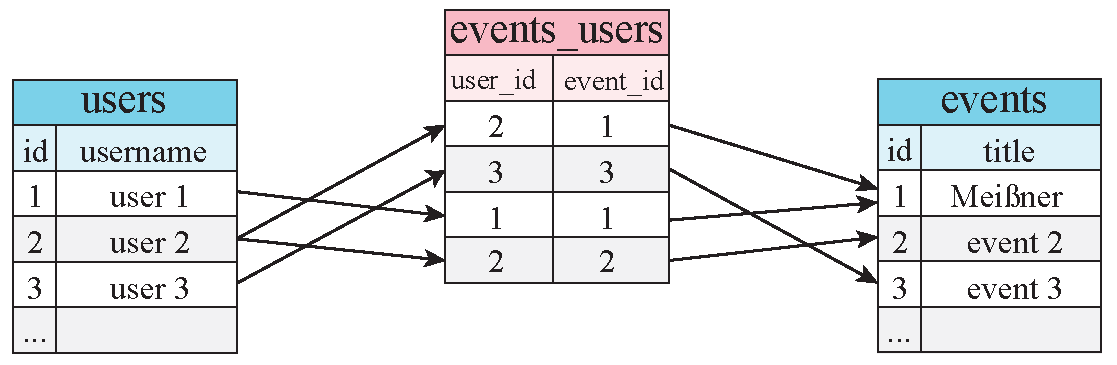
\includegraphics[width=15cm]{fig/events_users}
	\caption[Zuweisung eines Benutzers zu einer Veranstaltung]{Zuweisung eines Benutzers zu einer Veranstaltung (vereinfacht)}
\end{figure}

Diese \emph{Many-to-many}-Verknüpfung (in cakePHP auch \emph{hasAndBelongsToMany, HABTM} genannt) kann der EventsController mit einer einzigen SQL-Abfrage erfragen und erhält damit alle dem Event zugeordneten Benutzer. Diese Daten können dann in einer Variable gespeichert und dem View bereitgestellt werden.

\subsection{Veranstaltungsspezifische Eigenschaften}
Die ersten Schritte zu einer Webanwendung, die Veranstaltungen und Benutzer verwalten kann, sind nun erledigt. Bisher ist es allerdings nicht möglich in Veranstaltungen Felder zu definieren, die für eben jene Veranstaltung von Bedeutung sind. Das können im konkreten Fall Felder sein wie \glqq Art des Transportmittels\grqq{}, \glqq Wird ein Parkplatz benötigt?\grqq{}, \glqq Welcher Holzstangenbedarf besteht?\grqq{} oder Ähnliches.\par

\paragraph{Key-Value-Store} In einem Key-Value-Store wird die Datenbank mit den Werten (\emph{values}) über die Schlüssel (\emph{keys}) indexiert. Das hat den Vorteil, dass vorher nicht bekannt sein muss, welche Werte in die Datenbank eingetragen werden sollen. In der Meißner App wurde diese Methode implementiert, um eventspezifisch ein beliebiges Feld zu definieren, welches Werte als Strings annimmt.\\
So ist gewährleistet, dass die Benutzer dieser Anwendung die größtmögliche Freiheit besitzen, was die Inhalte der Veranstaltungen angeht. Jede kann individuell angelegt und personalisiert werden, sodass sie den gewünschten Anforderungen genügt.\\
Als Format für die Values wurden hier ausschließlich Strings gewählt, um den gesamten Vorgang zur Erstellung von speziellen Feldern möglichst gering zu halten. In der späteren statistischen Auswertung ist die Beschränkung des Feldes auf Strings irrelelevant, da sich diese sehr einfach beispielsweise mit PHP verwerten lassen.\par

\paragraph{Implementierung}
Für die Implementierung sind zwei weitere Tabellen notwendig: 

\begin{enumerate} 
	\item \emph{event\_columns}: Dient als Maske, um Feldnamen und -typen zu definieren. Kann innerhalb einer speziellen Veranstaltung genutzt werden, um diese Felder den zugeordneten Benutzern verfügbar zu machen.
	\item \emph{event\_properties}: Nachdem vom Controller die Feldnamen des Events abgefragt wurden, werden diese in einer Variable gespeichert und dem View übergeben. Im View wird dann ein Formular generiert, welches die Feldnamen aus \emph{event\_columns} anzeigt und die Möglichkeit gibt dort Werte einzutragen. Diese Werte werden dann über den Controller in \emph{event\_properties} gespeichert.
\end{enumerate}

Mit den Tabellen steht nun die Datenstruktur zur Verfügung, die es ermöglicht verantstaltungsspezifische Eigenschaften zu erstellen und die so erzeugten Feldern mit den entsprechenden Werten der Teilnehmer dieser Veranstaltung zu befüllen.

\begin{figure}[!ht]
	\centering
	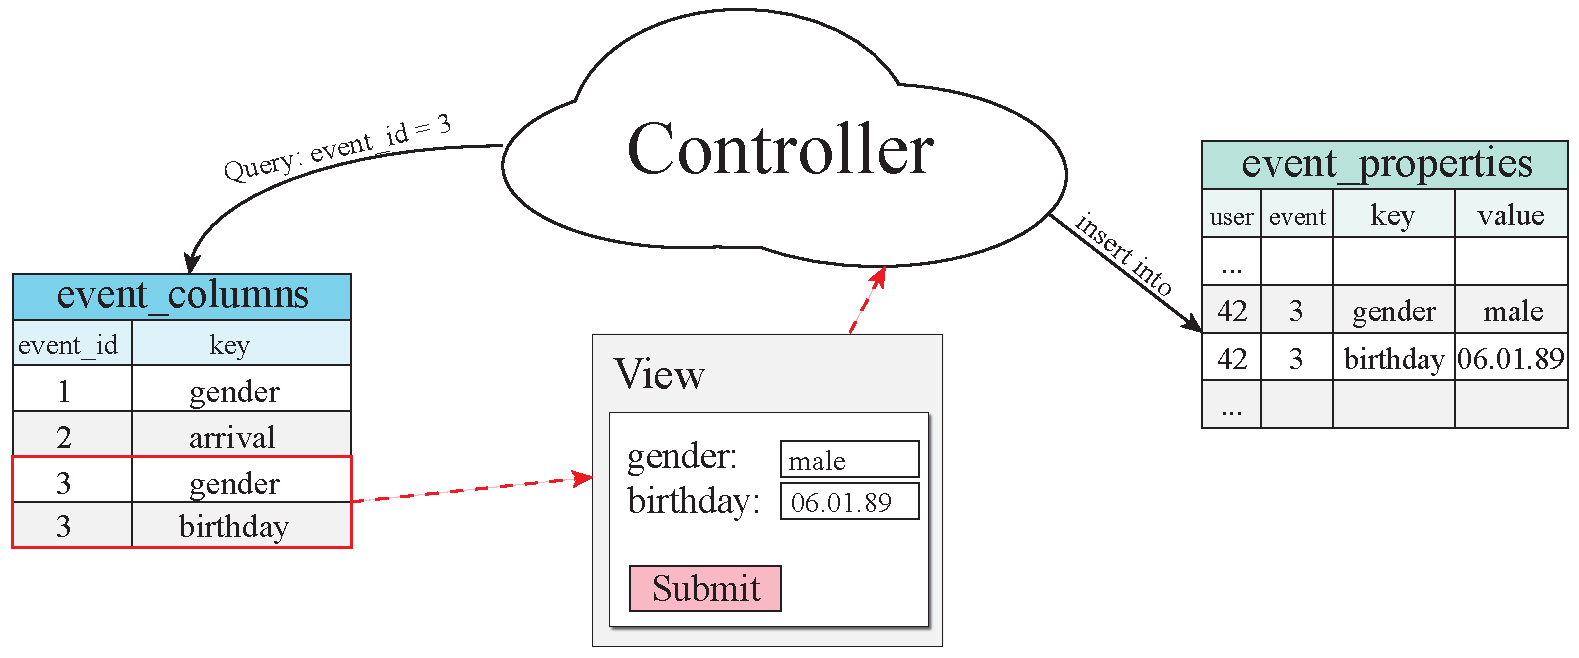
\includegraphics[width=15cm]{fig/event_properties}
	\caption[Speichern von spez. Feldern in die Datenbank]{Controller erfragt Felder aus event\_columns, stellt sie dem View zur Verfügung, speichert danach die Werte in event\_properties}
\end{figure}

Obige Abbildung zeigt kurz das Zusammenspiel von Controller und View: Datenbankzugriffe werden über den View an den Controller gerichtet und dort ausgeführt. So können Daten abgefragt oder neue Daten geschrieben werden.

\section{Views entwickeln}
Eine spannende Herausforderung ist es nun mit modernen Webtechnologien und möglichst geringem Aufwand direkt eine mobile Seite der Anwendung zu erstellen, welche für Smartphone und Tablets optimiert ist. Schließlich soll diese Web-App auch auf dem zugehörigen Platz mobil genutzt werden können.\par

Dabei gibt es mehrere Ansätze, wobei für diese Arbeit das sogenannte \emph{Responsive Webdesign} (deutsch: bedarfsgesteuertes Webdesign) für die mobile Version der Anwendung benutzt wird.

\subsection{Responsive Webdesign mit jQuery Mobile}
Hauptaugenmerk wird hier meistens auf die Auflösung des Endgeräts gelegt: Handelt es sich hierbei um ein günstiges Smartphone mit schlechtem Display, um ein Google Nexus 10 mit unglaublichen 2560x1600 Pixeln oder um einen SmartTV mit FullHD?\\
Diese Frage ist entscheidend, denn sie bestimmt wie viele und wie groß bestimmte Objekte im Sichtbereich des Geräts sein können, sodass der Benutzer nicht von der schlechten Bedienung genervt ist, sondern weiterhin die Informationen aus der App holen möchte. Beim Responsive Webdesign werden über \emph{Media Queries} (Abfrage der Eigenschaften des Geräts, Beispiel: Auflösung, Orientierung des Endgeräts usw.) Informationen des Endgeräts eingeholt und darauf abgestimmte Stylesheets geladen.\par

Um aber eine Webanwendung zu entwickeln, die aussieht und sich \glqq anfühlt\grqq{} wie eine echte App wurde in dieser Arbeit das Framework \emph{jQuery Mobile} verwendet, welches auch auf Responsive Webdesign setzt und dabei viele Steuerelemente zur Verfügung stellt, die dem Benutzer schon von nativen Apps her bekannt sind, wie typische Slider, Buttons, Dropdown-Menüs und vielem mehr.\par

So sind lediglich wenige Änderungen am normalen View nötig, um daraus eine mobile Version zu entwickeln, die für die Bedienung mit dem Finger optimiert ist.